\documentclass[ddcfooter,nosectionnum]{tudbeamer}
\usepackage{german}
\usepackage{graphicx}
\usepackage{listings}
\usepackage{setspace}
\usepackage{array}
\usepackage{wrapfig}
\usepackage{fontspec}
\usepackage{xltxtra}
\usepackage[font=scriptsize,labelfont=bf]{caption}

\setmainfont{Ubuntu}
\setmonofont{Courier}
\setromanfont{Ubuntu}
\setsansfont{Ubuntu}

\begin{document}

\einrichtung{Fakultät Informatik\hspace{6cm} Institut für Systemarchitektur}
\title[Speicherverwaltung in Linux]{Speicherverwaltung in Linux}
\subtitle{Proseminar Betriebssysteme}
\author{Rebecca Kratsch}

\date{10.05.2013}

\maketitle
	

\begin{frame}
    \frametitle{Inhalt}
	\tableofcontents
\end{frame}

\section{Grundlagen}
\begin{frame} 
    \frametitle{Grundlagen}
    	\begin{itemize}
			\item Physischer Speicher in Seiten strukturiert
			\begin {itemize}
				\item 32-bit Architektur meist 4Kb Seiten, 4 GB adressierbar
				\item 64-bit Architektur meist 8Kb Seiten, 16 Exabyte adressierbar
    		\end{itemize}
			\item Virtueller Adressraum je Prozess (auf 32-bit-Maschinen)
			\begin {itemize}
				\item 3 GB virtueller Adressraum: Text-, Daten-, BBS-Segment, Stapel			\item 1 GB: Seitentabellen und andere Informationen des Kerns    			\end{itemize}
    \end{itemize}
    \end{frame}


\begin{frame}
	\frametitle{Grundlagen}
    \framesubtitle {Gliederung eines Linux-Prozess-Adressraumes }
	
		\begin{table}
		\centering
			\begin{tabular}{*{2}{m{0.6\textwidth}}}
			\begin{itemize}
		 		\item Stack:  
				\begin{itemize}
					\item Umgebungsvariablen, Kommandozeile, lokale Variablen
					\item veränderbar
				\end{itemize}  	
				\item Datensegment:  
				\begin{itemize}
					\item initialisierte Daten    
					\item uninitialisierte Daten
				\end{itemize}
				\item Textsegment: 
				\begin{itemize}
					\item Maschinenbefehle
					\item nur lesender Zugriff
					\item keine Größenänderung mögl. 
				\end{itemize}
    		\end{itemize}
&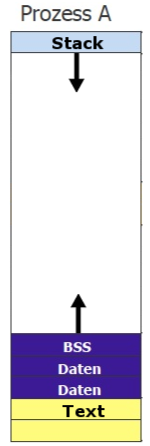
\includegraphics[width = 1.8cm]{segmente.png}
			\end{tabular}
			\label{tab:gt}
		\end{table}
\end{frame}


\begin{frame} 
    \frametitle{Grundlagen}
    \framesubtitle{Memory-Mapped-Dateien}
    \begin{figure}[p]  
    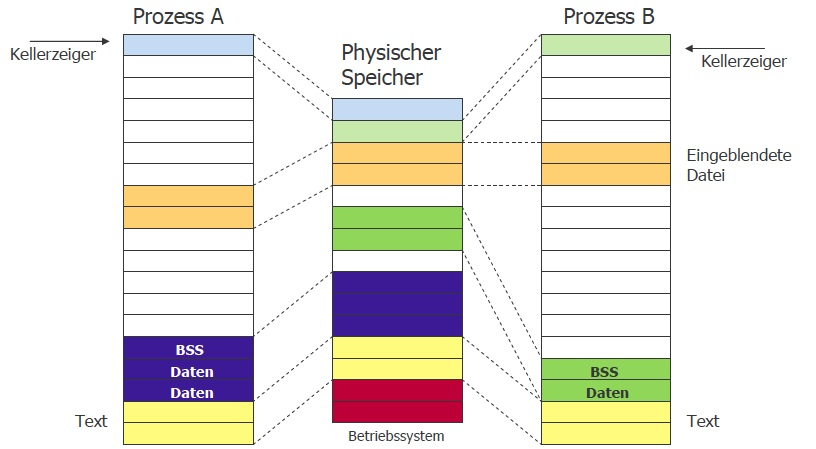
\includegraphics[width=9.3cm]{mmd.png}
    \caption{ Kao, O.; Vorlesung Betriebssysteme; Universität Paderborn; 2005}
     \end{figure}
\end{frame}



\section{Physischer Speicher}
\begin{frame}
    \frametitle{Verwaltung des Physischen Speichers}   
   	  \begin{itemize}
      	\item Unterscheidung von 3 Speicherzonen: 
		\begin{description}
					\item 1. ZONE\_DMA 
					\item 2. ZONE\_NORMAL
					\item 3. ZONE\_HIGHMEN
				\end{description} 

	  
			
			
%			\begin{tabular}{*{2}{m{0.5\textwidth}}}
%				\begin{description}
%					\item 1. ZONE\_DMA 
%					\item 2. ZONE\_NORMAL
%					\item 3. ZONE\_HIGHMEN
%				\end{description} &
%			\begin{figure}
%     
%      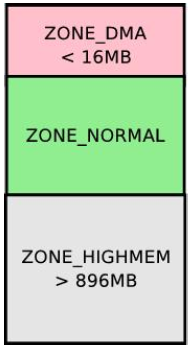
\includegraphics[width=2.5cm]{zonen.png}
%     \end{figure}
%	\end{tabular}
	
	\item Arbeitsspeicher 3 Teile: 
	\begin{itemize}
		\item Kern
		\item Speicherzuordnungtabelle
		\item restlicher Anteil: Aufteilung in Seitenrahmen
	\end{itemize}
	\end{itemize}
\end{frame}

\begin{frame}
	\frametitle{Verwaltung des Physischen Speichers}
    \begin{itemize}
    	\item Seitendeskriptoren
        \begin{itemize}
			\item Zeiger auf zugehörigen Adressraum
			\item Typ: \texttt{page}, Name: \texttt{mem\_map}
       	\end{itemize}
		\item Zonendeskriptoren
		\begin{itemize}
			\item Informationen für Speicherausnutzung jeder Zone
			\item Identifizierung freier Arbeitsspeicherbereiche durch
			\texttt{free\_area[]}
		\end{itemize}
		\item Knotendeskriptoren
		\begin {itemize}
			\item zur Differenzierung zwischen physischem Speicher auf verschiedenen Knoten	
			\item Informationen über Speichernutzung und Zonen des speziellen Knotens
		\end {itemize}			
   	\end{itemize} 

   
       
\end{frame}

\begin{frame}
	\framesubtitle{Mechanismen zur Speicherbelegung}
	\begin{itemize}
		\item\textbf{Page Allocator}unter Nutzung des Buddy-Algorithmuses
	
	\end{itemize}
	
	
\end{frame}	

\section{Virtueller Speicher}
\begin{frame}
    \frametitle{Virtueller Adressraum}
    \begin{itemize}
         \item   Unterteilung in homogene, zusammenhängende, an Seitengrenzen ausgerichtete 			Regionen
         \item fixe Seitengröße, erweiterbar durch PAE
        
     \end{itemize}
    
\end{frame}



\begin{frame}
    \frametitle{Virtuellen Adressraum}
    \begin{itemize}
    	    \item Beschreibung jedes Kernbereichs mit \texttt{vm\_area\_struct}-Eintrag 
   		\begin{itemize}
			 \item sortiert und zusammengefasst nach virtueller Adresse\\
			\item enthält Eigenschaften (Schutzrechte...)
			--> Realisiserung Copy- on-Write
			\item Angaben über Hintergrundspeicher
    			\item Zugriff auf alle Elemenete eines Adressraumes via Speicher-Deskriptor
			\begin{itemize}
				\item verkettete Liste
				\item binärer Rot-Schwarz-Baum
			\end{itemize}
   		\end{itemize} 
	\end{itemize}
    
\end{frame}

\begin{frame}
    \frametitle{Virtueller Adressraumes}
    \framesubtitle {Paging in Linux}
    \begin{itemize}
         \item  Grundeinheit: Seite
         \item Grundidee / Definition Paging: \\
        \begin{quote}
         „Paging ist ein Speicherverwaltungsverfahren, das auf der Strukturierung  des virtuellen Speichers 	in Seiten und der Strukturierung des realen Speichers in Seitenrahmen beruht.“
         \footnote{EHSES, E. u.a. : Betriebssysteme- Ein Lehrbuch mit Übungen zur Systemrogrammierung in UNIX/Linux. 3. Aufl. München: Pearson Studium Verlag, 2005, S.294}
	\end{quote}
 	
	
    
    
     \end{itemize}
    
\end{frame}


\begin{frame}
    \frametitle{Virtueller Adressraum}
    \framesubtitle {Paging in Linux}
    \begin{itemize}
         \item Nutzung 4-stufiger Seitentabellen in Linux\\
         --------Grafik überarbeiten ----------
	%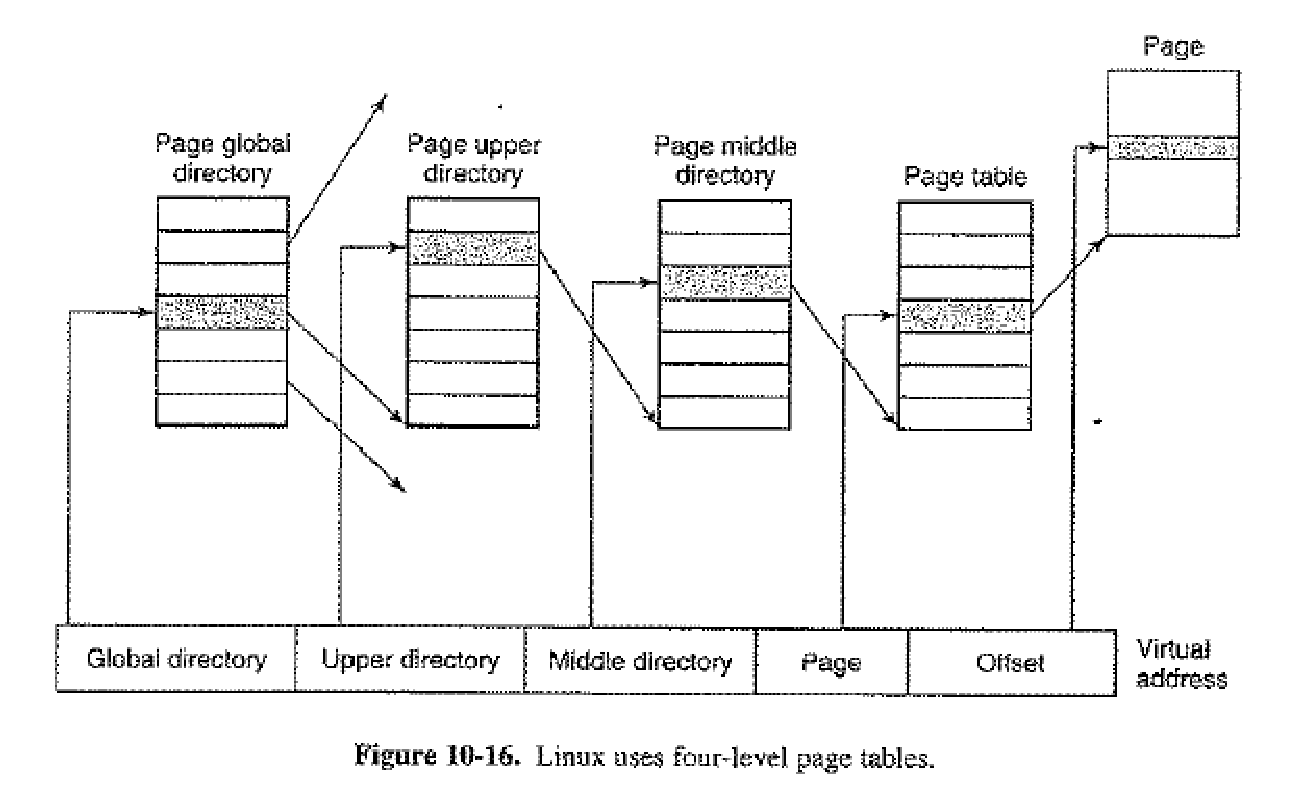
\includegraphics[width=6cm]{Seitentab.eps} 		
    
    
     \end{itemize}
    
\end{frame}


\begin{frame}
 
    \frametitle {Virtueller Adressraum}
    
    \framesubtitle {Paging in Linux}
    \begin{itemize}
         \item  Grundeinheit: Seite
         \item Grundidee / Definition Paging: \\
        \begin{quote}
         „Paging ist ein Speicherverwaltungsverfahren, das auf der Strukturierung  des virtuellen Speichers 	in Seiten und der Strukturierung des realen Speichers in Seitenrahmen beruht.“
     	 \end{quote}
 	 \item Nutzung 4-stufiger Seitentabellen in Linux
	 \item Realisierung sowohl durch kern als auch durch Page-Daemon
	 \item Demand - Paging - System unter Nutzung des Swap-Bereiches
	 \begin{itemize}
	 	\item Auslagerungspartitionen 
		\item Auslagerungsdateien
	\end{itemize}
    
    
     \end{itemize}
    
\end{frame}

\begin{frame}
	\frametitle{Virtueller Adressraum}\
	\framesubtitle {Der Seitenersetzungsalgorithmus}
 	\begin{itemize}
		\item per Page Frame Reclaiming Algorithmus
		\item Unterscheidung von vier Seitenarten:
	\end{itemize}	
		
		\begin{center}
		{\tiny
		\begin{tabular}{ l l }
 			 unreclaimable :&  reserviert/gesperrt/nicht auslagerbar \\
  			 swappable:       &  zurück auf Swap bzw Auslagerungspartition vor Neuanforderung\\
 			 syncable:		 &  zurück auf Platte, falls verändert\\
			 discardable:      & sofort anforderbar\\
		\end{tabular}
		}
		\end{center}
		
		zu beenden

			
    
\end{frame}



\section{Zusammenfassung}
\begin{frame}
    \frametitle{Zusammenfassung}
    \begin{itemize}
         \item   
    
    
    
     \end{itemize}
    
\end{frame}


\section{Literatur}
\begin{frame}
    \frametitle{Literatur}
    \begin{itemize}
         \item  Moderne Betriebssysteme \\
        		Andrew S. Tanenbaum - 2010
	\item	 UNIX - Wie funktioniert das Betriebssystem? \\
		Maurice J. Bach - 1991
	\item Betriebssysteme\\
		EIn Lehrbuch mit Übungen zur Systemprogrammierung in UNIX/ Linux \\
		E.Ehses, L. Köhler, P. Riemer, H. Stenzel, F. Victor - 2010	
    \end{itemize}
    
\end{frame}

\end{document}






